% !TeX root = ../thesis.tex
\section{Performance explorations}
\subsection{Shared Memory}\label{subsec:sharedmem}
Reducing use of register could open up for higher thread-configuration for some plans and may make kernels execute faster even if 32 or less registers were used (see section \ref{subsubsec:occupancy}).
As the fastest general purpose alternative to registers, shared memory is the only real alternative type of memory.
As shared memory requires array-allocation for the entire block of threads, it does require the kernel to know how many threads per block there will be during kernel compilation.
This is no big sacrifice as this was indirectly a requirement for the parameterized solutions in any case.
Another limitation is the total size of the shared memory which is 48KiB per SM.

The elements that could be moved to shared memory are the parameter arrays and the temporary arrays used by the Runge-Kutta 4 solver.
A working copy of the result array could also potentially be moved to shared memory, but it would still require the result array to be copied back to global memory at some point.
It is unlikely that this would lead to an increase in performance.
The $Va$ array is also only read from once and is unlikely to be a good candidate to copy to shared memory.

As a big source of local memory used was the temporary arrays $k1$, $k2$, $k3$, $k4$, $tmp$ and $v$ with the number of states in the plan as the size, these were moved to shared memory.
It is worth noting some properties of the kernels for the various plans before and after.
The number of registers can be seen in table \ref{table:tempArraysSharedMemory}.
It is interesting to see that the storing the temporary arrays in local memory actually uses the least registers for single precision floats, considering that the temporary arrays should no longer be stored in them.
It is possible that it is using the added registers as a cache for accessing the shared memory.
It is also interesting that marking the memory as volatile - meaning that the compiler should not optimize reads and writes for the array - reduces the register usage slightly for single precision floats.
It also reduces the number of registers a more significant number for doubles, almost to the point that 1024 threads per block can be used.

\begin{table}[h!]
\centering
{\setlength{\extrarowheight}{2pt}{\setlength{\tabcolsep}{3pt}
\begin{tabular}{ | l | r | r | r | r | r | r | }
  \hline
								&	L32		&	S32			&	S32v		&	L64		&	S64			&	S64v	\\ \hline
Pure Endowment					&	20		&	22			&	22			&	32		&	33			&	29			\\ \hline
Deferred Temporary Life Annuity	&	19		&	24			&	23			&	34		&	35			&	30			\\ \hline
Temporary Life Annuity Premium	&	19		&	24			&	23			&	34		&	35			&	30			\\ \hline
Term Insurance					&	20		&	24			&	24			&	34		&	35			&	30			\\ \hline
Disability Annuity				&	25		&	26			&	25			&	45		&	46			&	34			\\ \hline
Disability Term Insurance		&	25		&	27			&	26			&	46		&	46			&	34			\\ \hline
\end{tabular}}}
\caption{Register usage using various types of memory for the temporary arrays in the parameter-less Runge-Kutta 4 solver. L = local memory, S = shared memory, 32 = single precision floats, 64 = double precision float, v = volatile memory.\label{table:tempArraysSharedMemory}}
\end{table}

Another aspect is the range to which shared memory can be used.
With a hard limit of 48KiB of shared memory per SM, divided by these six temporary arrays with size of the number of states divided by four bytes for single precision floats and eight bytes for double precision floats, the following number of total states is the following:
\begin{itemize}
\item Single precision floats allow for 2048 states (for example 1024 threads with two states).
\item Double precision floats allow for 1024 states (for example 512 threads with two states).
\end{itemize}

This does limit the applicability of shared memory, especially as life insurance policies can use significantly more states (for example the GF810 plan, see section \ref{subsubsec:gf810parallelized}).
To get around this, either runtime configurations with a low number of threads per block will have to be used, or only a subset of the temporary arrays can be moved to shared memory.

The results of moving the temporary arrays to shared memory resulted in a 12.24\% increase in runtime for single precision which more than doubled when also marking the arrays as volatile.
This is somewhat understandable as the single precision floats did not use a lot of registers to begin with and shared memory is generally slower than registers.
When marking the arrays as volatile, the runtime increases by 24.74\% compared to the original solution.
For double precision floats the situation is slightly different as it used a lot of registers, and it achieved a negligible (0.45\%) decrease in runtime.
Marking the arrays as volatile turned this into a 7.72\% increase instead.
All in all not very impressive for the simple example life insurance plans.

If instead we turn to a more advanced life insurance plan such as the limited implementation of the GF810 (see section \ref{sub:gf810}) which uses 50 states, the results look a bit different.
As there are nowhere near enough registers for 50 states, the remaining states need to be stored in local (global) memory which is slow.
For double precision floats it ends up using all 63 available registers per thread and spills 8568 bytes to local memory.
With 50 states, only up to 20 threads per block (less than a warp) worth of shared memory is available, regardless the results seem positive.
Where execution using local memory takes about 5.52 seconds, using volatile shared memory takes only 3.97 seconds making it 27.66\% faster.
Non-volatile memory is slightly slower at 4.30 seconds, but still with an improvement of 21.53\% compared to local memory.
It is somewhat surprising that the volatile memory is faster, as the kernel claims to use more local memory and an identical amount of shared memory as the non-volatile.
Why this is so is yet unknown.

For all the shared memory results see appendix \ref{app:shared_memory}.

\subsubsection{Occupancy}\label{subsubsec:test:occupancy}
Occupancy (see section \ref{subsubsec:occupancy}) is a term used to describe how optimally the GPU is utilized with regards to warps, and is affected by the number of threads per block, shared memory per block and registers per thread.
The method of limiting registers in Alea.cuBase did not work and as the Runge-Kutta 4 solver results in many different numbers of registers based on the life insurance plan, there is no general way of ensuring register limits.
The solver also only has limited changeable aspects with regards to registers and shared memory is subject to the number of states a given insurance plan uses.
This results in the only reliably changeable aspect being the number of threads per block subject to registers and shared memory usage of the kernel.

Testing showed that lower thread configurations often had low occupancy (not surprising), and higher thread configuration typically reached 67\% which many find is enough to saturate the bandwidth (see section 10.4 of \cite{cudacoccupancy}).

\subsection{Expression reduction}\label{subsec:exprReduction}
Alea.cuBase claims to generate highly optimized CUDA code so simple kernel optimization might be a futile effort.
Nonetheless an optimization method $optimize$ was written which performs fairly simple arithmetic reductions.

It is based on recursive pattern matching that performs the following operations:
\begin{itemize}
\item If working with a non-arithmetic expressions such as a $Let$ or $Lambda$-expressions, call $optimize$ on its components
\item If working with a binary arithmetic expression, call $optimize$ on its components and reduce based on the following rules:
	\begin{itemize}
	\item If working with an expression where both components evaluate to numbers, simply evaluate and return the number. This applies to both addition, subtraction, multiplication and division.
	\item If working with addition where one of the components is zero, return the non-zero component.
	\item If working with subtraction where the first component is zero, return a negation expression of the second component.
	\item If working with subtraction where the second component is zero, return the first component.
	\item If working with multiplication where either component is one, return the other component.
	\item If working with multiplication where either component is zero, return zero.
	\item If working with division where the first component is zero, return zero.
	\item If working with division where the second component is one, return the first component.
	\end{itemize}
\end{itemize}
It does one additional reduction which removes empty ($() : unit$) elements of a $Sequence$ of Expressions.

Comparing an optimized version to a non-optimized version shows an overall runtime reduction of about 2.39\% for single precision floats and 1.46\% for double precision.
See appendix \ref{app:optimization_performance} for all the timing results.

The fact that these simple reductions reductions improve the runtime of reasonable efficient kernels makes the reduction seem worthwhile.
As life insurance plans in CalcSpec can both be more advanced and unoptimized, this becomes particularly relevant.

Further possible reductions could include removing unreferenced let-declarations as well as more numerical and arithmetic reductions.
There are also more possible numerical reductions, as the first rule only works for the end of an expression ($... 5 - 10$) and otherwise not ($... 5 - 10 + t$).

\subsection{Collective Spouse Pension}\label{sub:gf810}
The collective spouse pension (``grundform 810'' or GF810 in Danish) is a life insurance policy in which upon the death of the ensured, the spouse receives a life annuity, if one such exists.

\subsubsection{Traditional method of computation}
GF810 is traditionally calculated as a 3-tier process with an outer, middle and inner model.

The \emph{outer model} can be seen as a 2-state (active-dead) Markov-model where the transition cost to the death state is the \emph{middle model}, solved from 120 minus the age of the ensured to 0.
The \emph{middle model} can be seen as another 2-state Markov-model, but rather than using Thiele's equation it calculates \lstinline$-gp(tau) * h(eta, tau) * Inner(eta, k, t)$ where $gp$ is the marriage-probability of a $tau$-aged individual and $h$ is the probability that a $tau$-aged individual is married to an $eta$-aged individual given that the first individual is married.
This is solved from 120 to 1. The middle model can also be solved using numerical integration.
The \emph{inner model} is another 2-state Markov-model with benefit paid being $indicator(s >= k)$ (indicator returns one if true, otherwise zero) and transition intensity being the spouse death mortality intensity, solved from 120 minus $eta$ to 0.

It is a fairly complex method of computation as is also apparent in its execution time which takes up to two and a half minutes on the CPU.
While the traditional method of computation can be run on the GPU as-is, it is not particularly suited for it due to the long time it takes to execute and as there is a lot of code branching making threads finish at very different times making them less efficient to execute in parallel.

\subsubsection{Parallelized method of computation}\label{subsubsec:gf810parallelized}
An alternative approach was suggested by Klaus Grue of Edlund using a single-tier approach.
The Markov-model contains the active state for the insured, 125 intermediary states signifying death of the insured when married to a spouse of an age difference from -62 to +62 and a final state signifying either death of the spouse or death of the ensured when unmarried, as depicted in figure \ref{fig:gf810}.

\begin{figure}[h!]\centering
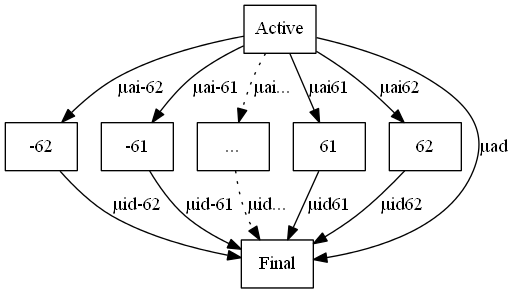
\includegraphics[scale=0.5]{gf810.png}
\caption{Markov-model for the parallelized GF810 Artificial Collective Spouse Pension plan.\label{fig:gf810}}
\end{figure}
\newcommand*{\diff}{\ensuremath{\mathit{diff}}}
The transition probability to one of the intermediary states $\mu_{ai}$ is the mortality intensity for the ensured at time $t + age$ times the marriage probability that a $t + age$ year old is married to a $t + age + \diff$ year old where $\diff$ is the age difference of the spouse and the ensured as well as the number of the state.
The ensured to final state $\mu_{ad}$ probability is the mortality intensity of the ensured at time $t + age$ times the probability that the ensured is not married at time $t + age$ (1 minus the marriage probability at the time).
The intermediary to final state $\mu_{id}$ probability is the mortality intensity of the spouse at the time (assuming the sexuality of the ensured does not change) of age $t + age + \diff$.

This does potentially lead to a lot of cases where the ensured will either be married to someone yet to be born or someone significantly older than the oldest person alive today, which can be a problem for the Gompertz-Makeham mortality intensity methods.
To lessen the impact of this, the result of these functions is constrained to be no higher than two by adding a constraint method.

This model of calculation can already be expressed in CalcSpec as is, but is somewhat cumbersome to write as there is little variability in the model.
The final CalcSpec should resemble code sample \ref{gf810cs}.
Note that the \lstinline$\var.expr$ is CalcSpec syntax for lambdas. 
It is currently also required to update the $from$ value in the $range$ section to the value of 120-age, as this is currently not possible to have variable values for this in the current solution.

\begin{lstlisting}[language=calcspec, caption=GF810 full CalcSpec, label=gf810cs]
calculation = {
  name = "GF810 - Collective spouse pension", 
  algorithm = { type="Runge Kutta 4", parameters={ stepsize = 0.01 }}, 
  equations = { 
    0 = { r_j = rate, b_j = 0, mu_jk = { 
        1 = mu_ai(-62), 2 = mu_ai(-61),
        ...,
        124 = mu_ai(61), 125 = mu_ai(62), 
        126 = \t.(GM_f(t)) * (1 - gp(t + age))
      }, b_jk = {  } }, 
    1 = { r_j = rate, b_j = 1, mu_jk = { 126 = mu_id(-62) }, b_jk = {}}, 
    2 = { r_j = rate, b_j = 1, mu_jk = { 126 = mu_id(-61) }, b_jk = {}}, 
    ...,
    124 = { r_j = rate, b_j = 1, mu_jk = { 126 = mu_id(61) }, b_jk = {}}, 
    125 = { r_j = rate, b_j = 1, mu_jk = { 126 = mu_id(62) }, b_jk = {}}, 
    126 = {  } }, 
  range = { from = 85, to = 0 }, 
  boundaryvalues = { 0 = 0, 1 = 0 }, 
  expressions = { 
    interestrate = 0.05, 
    age = 35, 
    rate(t) = interestrate, 
    GM_f(t) = constrain(0.0005 + 10 ^ (5.728 - 10 + 0.038 * (age + t))), 
    GM_m(t) = constrain(0.0005 + 10 ^ (5.88 - 10 + 0.038 * (age + t))), 
    mu_ai = \diff.\t.GM_f(t) * gp(t+age) * (h(t+age+diff)(t+age)), 
    mu_id = \diff.\t.GM_m(t + diff) 
  }
}
\end{lstlisting}

To optimize this process, functionality was added to transform the CalcSpec AST based on the variability of the GF810 plan.
See code sample \ref{gf810simplifiedcs} for an example of this which is converted back to the code in code sample \ref{gf810cs}.

\begin{lstlisting}[language=calcspec, caption=GF810 simplified CalcSpec, label=gf810simplifiedcs]
calculation = { 
  name = "GF810 - Collective spouse pension", 
  algorithm = { type="Runge Kutta 4", parameters={ stepsize = 0.01 }}, 
  equations = { 
    GF810 = { age=age, rate=rate, mu_insured=GM_f, mu_spouse=GM_m }
  }, 
  range = { from = 85, to = 0 }, 
  boundaryvalues = { 0 = 0, 1 = 0 }, 
  expressions = { 
    interestrate = 0.05,
    age = 35,
    rate(t) = interestrate,
    GM_f(t) = constrain(0.0005 + (10 ^ (5.728 - 10 + 0.038 * (age + t)))),
    GM_m(t) = constrain(0.0005 + (10 ^ (5.88 - 10 + 0.038 * (age + t))))
  }
}
\end{lstlisting}

\subsubsection{Issues}
When attempting to compile the generated kernel with Alea.cuBase, an unexpected stack overflow exception was thrown during kernel compilation by Alea.cuBase.
By reducing the range of intermediary states from -62...+62 to -24...+24 for double precision and -36...+36 for single precision it was compilable again.

Various changes were made hoping to increase the maximum number of intermediary states but to no avail.
They consisted of the following:
\begin{itemize}
\item Reducing the depth of the generated AST. This included using a sum variable for the various state transitions as well as expression reduction by the $optimize$ method described in section \ref{subsec:exprReduction}.
\item Reducing the local memory used by moving the temporary arrays to shared memory.
\end{itemize}

\subsubsection{Results}
As the Alea.cuBase solution did not support the required number of states a CPU-version was implemented to test the validity of the new method.
For age 35 it provided identical results down to the 7th decimal and as a bonus it completed in 1060 ms on average - an improvement of close to factor 150.
Another interesting fact is that for age 35, the limited 50-states Alea.cuBase solution with intermediary states from -24...+24 was also identical down to the 7th decimal, and to the 10th decimal compared to the -62...+62 CPU version.
The sum of the reserve at every year also only leaves a relative difference of about 0.02\%, while the relative difference of the final result (year zero) is only $9.733035931 \cdot 10^{-7}\%$.
The relative difference of the sum of the reserves for the GPU version with all intermediary states stays under 0.09\% for tested ages up to 80, with the relative difference of the final result only reaching $6.107283993 \cdot 10^{-6}$\%.

This is sadly not a feat the limited 50-states implementation can claim to achieve. 
With age 15 there is a 9.45\% relative difference in the final result while at age 50 there is a 68.34\% relative difference.
For a visualization of this, see figure \ref{fig:gf810ages}. 
Note that many of the entries can not be seen as they are overlapping due to being practically identical.
The cause of the results getting progressively worse as the age increases is due to the fact that the marriage-probability in the early years is incredibly small.
It is also because as the insured grows older, the younger spouses account for a lot more of the reserve than older spouses that die earlier.
Since there is not enough intermediary states to reach these young spouses, the results are skewed.

\begin{figure}[h!]\centering
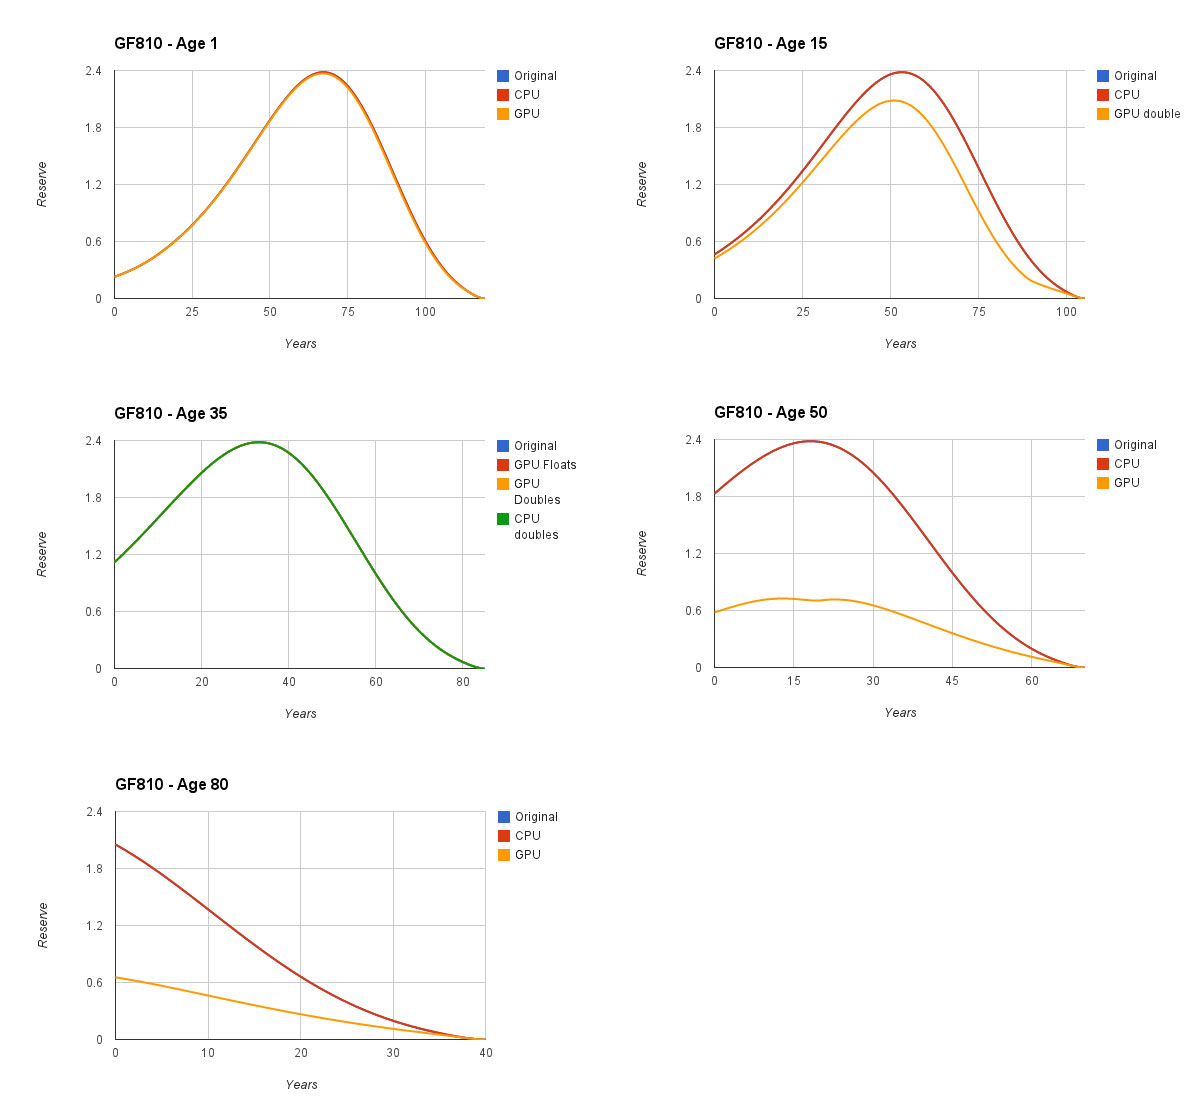
\includegraphics[scale=0.3]{GF810-ages.jpg}
\caption{Comparison of GF810 reserve-output for ages 1, 15, 35, 50 and 80 using results from the original solution, a CPU-version of the new method and the limited state GPU-version of the new method.\label{fig:gf810ages}}
\end{figure}

To conclude, the method definitely works in theory even if not currently on the GPU.
It does require all the intermediary states unless certain ``sweet spots'' are hit, which can not be relied upon.

Speed-wise, it is hard to compare running-times without being able to utilize all the required states.
For the limited 50-states version with intermediary states from -24...+24, tests were performed in section \ref{subsec:sharedmem} which resulted in runtimes of 5.52 seconds using global memory, 3.97 seconds using volatile shared memory and 4.30 second using non-volatile shared memory, but especially the shared memory results are inaccurate for the full solution as there is simply not enough shared memory available for all states.
If not using shared memory (or at least no more than 96 bytes per thread), 512 threads per block would still be an option.
This would result in the remaining registers spilling to local memory which would decrease performance.
An optimist could claim that similar relative increases as seen in simpler plans could be achieved, which would still be a massive performance increase.
A pessimist could argue that the use of slow local memory and overall complexity would limit the performance significantly.
No matter which camp you might be in, it is very likely that given enough iterations there should still be a significant increase in performance when calculating a large enough number of iterations.

For double precision comparison results, see appendix \ref{app:gf810ageresults}.

\subsubsection{Step-size experimentation}
A straight-forward way to increase performance is to reduce the number of steps used by the Runge-Kutta solver at the cost of increased error.
This was tested on the CPU-implementation of the new GF810 method with 16, 32 and 64 as the number of steps compared to the original 100 steps, and tested for ages 10 to 100 in 5 year intervals.

Results showed that with just 16 steps an average relative error compared to 100 steps was no more than $6.18318 * 10^{-11}$ with an increase in performance of factor 6.24.
For 32 as the number of steps the error was reduced to $6.3476 * 10^{-12}$ with an increase in performance of factor 3.13, and for 64 as the number of steps, the error was reduced to $1.626 * 10^{-12}$ with an increase in performance by factor 1.57.

One important trend to note is the fact that as age increases, and as a result the years calculated decreases, the rate of error increases.
As the high-age calculations already require less computation it would be ideal to use larger step-sizes for these computations.

For the results of the various step-sizes, see appendix \ref{app:gf810stepsizes}.

